\subsection{Centroid-based Clustering}
\label{centroid_clustering}
In analyzing the dataset using centroid-based methods, we experimented with two different algorithms, K-Means and Bisecting K-Means.
For each experiment, we followed the same steps:
\begin{enumerate}
    \item Choosing the attributes and scaling the dataset: we used all numeric features (cf. Table \ref{tab:dataset_numeric}), log-transformed if necessary as detailed in Subsec. \ref{numeric_vars_analysis}, and scaled the values using StandardScaler. %TO JUSTIFY STANDARDSCALER IN THE SUBSECTION INTRO, SINCE WE USED IT FOR ALL ALGORITHMS.
    \item Selecting the best value for \textit{k}: we used both the Elbow method and the Silhouette method as heuristics to determine the appropriate number of clusters. To do so, we iteratively run the algorithm for \textit{k} in the range [2,50], plotting the SSE and Silhouette score for each \textit{k} and comparing the two curves to find the best trade-off.
    \item Fitting the algorithm and evaluating the resulting clustering in terms of cohesion and separation by calculating the SSE, Silhouette score, and correlation between the distance matrix of the dataset and the ideal similarity matrix.
    \item Visual cluster exploration: cluster visualization through PCA, t-SNE, and a parallel coordinates plot of the centroids, followed by a further visualization of the clusters' composition w.r.t. categorical and numeric features.
\end{enumerate}

\subsubsection{K-Means}
We select k=7 as a trade-off between SSE and Silhouette score.
The resulting SSE and Silhouette score are 62588.082 and 0.189, respectively, while the correlation is -0.458. Though the SSE value might seem high, it is significantly lower than the SSE of 500 randomly generated datasets (cf. Figure \ref{fig:SSE_eval_kmeans.png}), which suggests that our clustering is meaningful and not a product of chance.

%\begin{figure}
%    \includegraphics[width=\columnwidth]{../results/images/elbow_kmeans.png}
%    \caption{SSE and Silhouette score for choosing \textit{k} (K-Means)}
%    \label{fig:elbow_kmeans.png}
%\end{figure}

\begin{figure}
    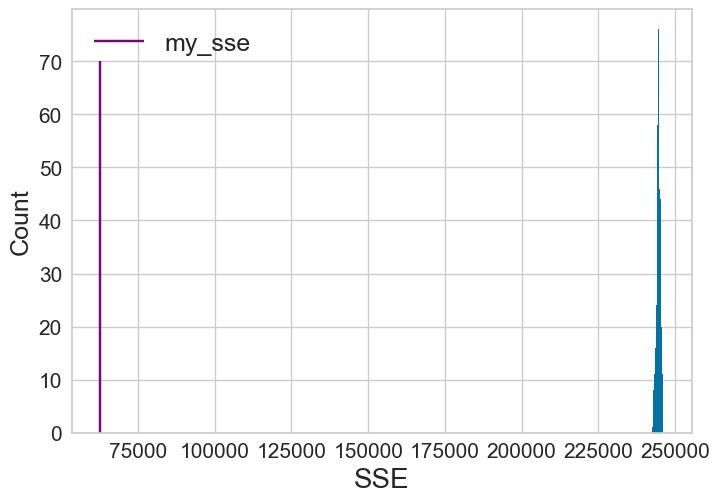
\includegraphics[width=\columnwidth]{../results/images/SSE_eval_kmeans.png}
    \caption{Statistical framework for clusters' validity: see (K-Means).}
    \label{fig:SSE_eval_kmeans.png}
\end{figure}

The clusters' composition is reported in Table \ref{tab:clusters_kmeans}: in terms of population, we can distinguish Cluster 0 as the largest cluster, with almost 5000 records, followed by Cluster 2 with over 3000 records. The smallest cluster is Cluster 6, with only 950 records. The remaining clusters have between 1400 and 2000 records.

The first thing that emerges from the parallel coordinates graph (Figure \ref{fig:centroids_kmeans.png}) is how Cluster 3 is well-separated from the others w.r.t half of the features: it has a particularly high value for \textit{numVotes}, \textit{totalImages}, \textit{totalCredits}, and \textit{numRegions}  – variables for which we had observed moderate correlation in Subsec. \ref{var_correlation_elimination} . Cluster 5 has a significantly higher value for \textit{criticReviewsRatio}: the algorithm might have isolated titles with greater critical appeal. Clusters 6 and 4 have the lowest runtime by far; Cluster 6, the smallest one, is also characterized by a low value for \textit{startYear} and \textit{totalCredits}: it probably contains the oldest and shortest titles. Clusters 0 and 2 appear to be the least-well separated from the others; they are indeed the biggest clusters. 

\begin{figure}
    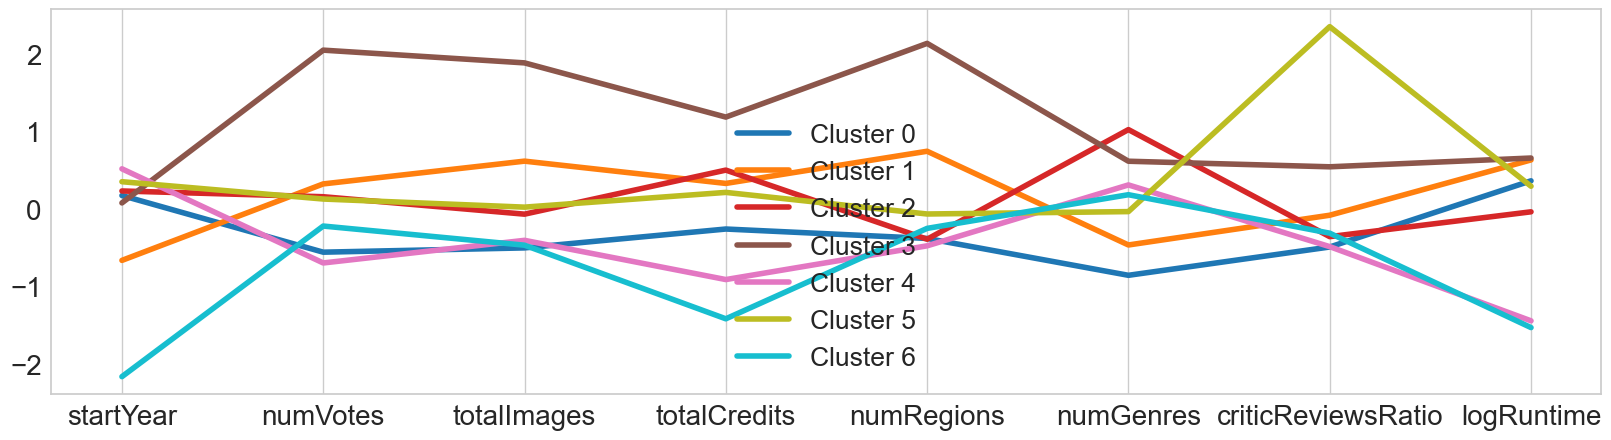
\includegraphics[width=\columnwidth]{../results/images/centroids_kmeans.png}
    \caption{Centroids' visualization for K-Means.}
    \label{fig:centroids_kmeans.png}
\end{figure}

\begin{table}[h]
    \centering
    \small
    \begin{minipage}{0.45\linewidth}
        \centering
        \begin{tabular}{|c|c|}
            \hline
            \textbf{Clust.} & \textbf{\# of records} \\ \hline
            0 & 4841 \\ \hline
            1 & 1985 \\ \hline
            2 & 3424 \\ \hline
            3 & 1424 \\ \hline
            4 & 1985 \\ \hline
            5 & 1822 \\ \hline
            6 & 950 \\ \hline
        \end{tabular}
        \caption{Clusters for K-Means.}
        \label{tab:clusters_kmeans}
    \end{minipage}
    \hfill
    \begin{minipage}{0.45\linewidth}
        \centering
        \small
        \begin{tabular}{|c|c|}
            \hline
            \textbf{Clust.} & \textbf{\# of records} \\ \hline
            0 & 1881 \\ \hline
            1 & 1398 \\ \hline
            2 & 1397 \\ \hline
            3 & 1712 \\ \hline
            4 & 3595 \\ \hline
            5 & 4184 \\ \hline
            6 & 2264 \\ \hline
        \end{tabular}
        \caption{Clusters for BK-Means.}
        \label{tab:clusters_bkmeans}
    \end{minipage}
\end{table}

In order to evaluate the results, we first used stratified bar charts to visualize the distribution of the clusters against known categorical features.
\begin{itemize}
    \item \textit{titleType} (cf. the heatmap in Figure \ref{fig:heatmap_titleType_kmeans.png}): the smallest cluster, Cluster 6, is the purest, being mainly made up of shorts. Nevertheless, it's Cluster 4 that contains the largest number of shorts (as well as some tvEpisodes). It also stands out for having the fewest movies – a class otherwise well represented across all other clusters. Cluster 2 has a very large proportion of tvEpisode, which explains its centroid's medium-low position for runtime in the parallel coordinates plot. The importance of \textit{logRuntime} for explaining this clustering is also highlighted by the fact that the few tvShorts present have been almost entirely distributed amongst these three clusters. Cluster 0, the biggest, contains a great number of almost all title types.
    \item Boolean variables: for almost all clusters, the True records represent a small proportion, except for Cluster 3: around half of its records are True for \textit{hasVideos} and \textit{awardsAndNominations}. Given the insights from the parallel coordinates plot, we can assume this cluster contains mainstream, popular content: it has relatively more videos, images, and votes on its page and was distributed in more countries, but it doesn't have the highest ratio of critical reviews. Cluster 6, on the other hand, has little to no True values for these variables. The highest proportion of True values for \textit{canHaveEpisodes} is in Cluster 0, which contains the largest amount of tvSeries and tvMiniSeries.
\end{itemize}

\begin{figure}
    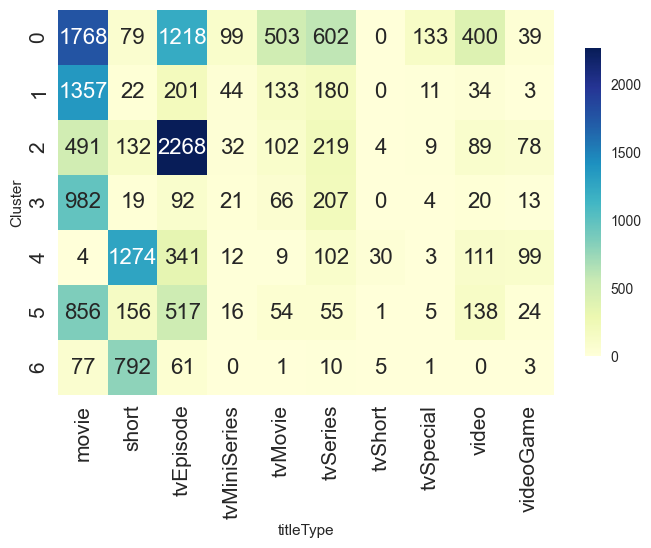
\includegraphics[width=\columnwidth]{../results/images/heatmap_titleType_kmeans.png}
    \caption{Heatmap Clusters vs titleType for K-Means.}
    \label{fig:heatmap_titleType_kmeans.png}
\end{figure}

We also analyzed the clusters' composition w.r.t. the numeric variables used by the algorithm, expanding the insights gained from the parallel coordinates plot.
Interestingly, the two purest clusters w.r.t to \textit{numGenres} are the biggest: Cluster 0 mostly has one genre, with a minority of two genres, while Cluster 2 mostly has three genres, with a small proportion of two genres. The other clusters are more heterogeneous, having all three possible values. 
The line graph in Figure \ref{fig:startYear_kmeans.png} shows the distribution of the clusters w.r.t. \textit{startYear}: as hinted by its centroid, Cluster 6 contains the majority of records released before 1930s, and has no record released after 1983. On the other hand, Cluster 4 only has records released since 1963: the algorithm has therefore grouped older shorts in a cluster and newer shorts in another. Cluster 1, which also had a relatively low centroid, mostly contains records from the 1930s until the 1990s.
Boxplots for the remaining variables also confirm the insights that were previously discussed. For \textit{runtimeMinutes}, Clusters 4 and 6 have the lowest median, at 12 minutes, as well as a short box, indicating low variability. Cluster 4 follows at 40 minutes, coherently with the lenght of a tvEpisode.
\begin{figure}
    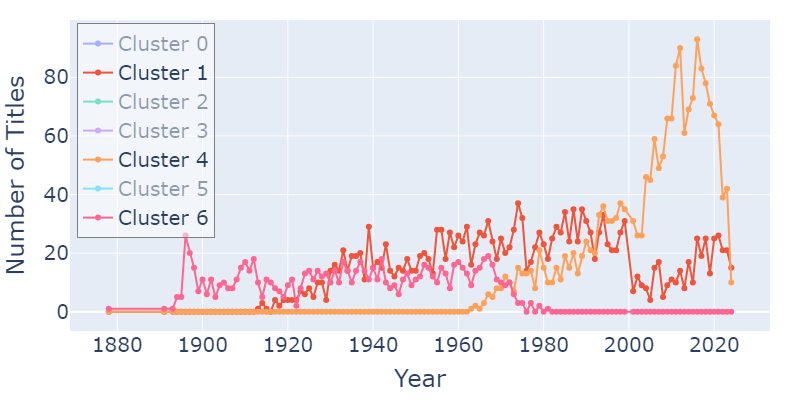
\includegraphics[width=\columnwidth]{../results/images/startYear_kmeans.png}
    \caption{Number of titles by year for relevant clusters for K-Means.}
    \label{fig:startYear_kmeans.png}
\end{figure}

\subsubsection{Bisecting K-Means}
We select k=7, the only significant local peak in the Silhouette plot (Figure \ref{fig:elbow_bkmeans.png}). All evaluation metrics are worse than the ones for K-Means, with a SSE equal to 67857.023, a Silhouette score equal to 0.128, and a correlation of -0.393. Again, we compared the SSE with the one of 500 randomly generated datasets to confirm its meaningfulness.
The clusters' sizes are more homogeous than K-Means' (cf. Table \ref{tab:clusters_bkmeans}): Cluster 5 is the biggest with around 4000 records, followed by Cluster 4 with almost 3600 records. All other clusters range between around 1400 and 2300 records.

\begin{figure}
    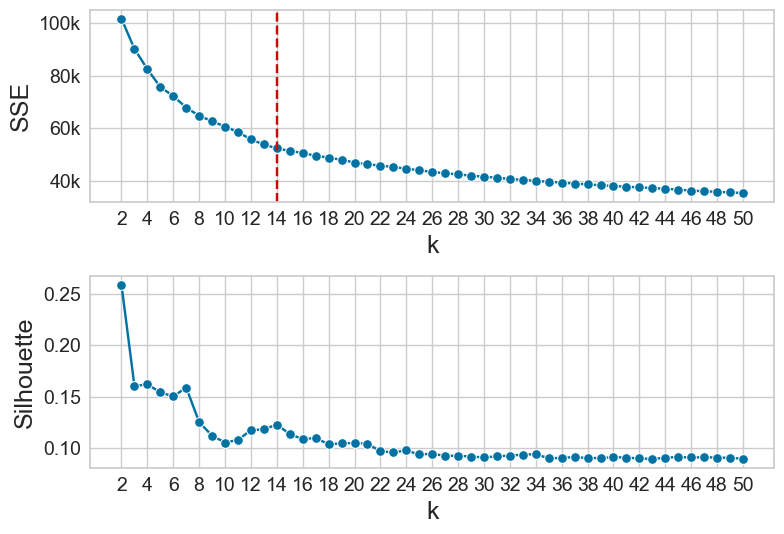
\includegraphics[width=\columnwidth]{../results/images/elbow_bkmeans.png}
    \caption{SSE and Silhouette score for choosing \textit{k} (BK-Means).}
    \label{fig:elbow_bkmeans.png}
\end{figure}

Analyzing the parallel coordinates plot in Figure \ref{fig:centroids_bkmeans.png}, we can see that similarly to before, there's a cluster, Cluster 2, that is well-separated from the others w.r.t. \textit{numvotes}, \textit{totalImages}, \textit{totalCredits} and \textit{numRegions}. In terms of these values, it is followed by Clusters 0 and 1. Moreover, there's once again a cluster, Cluster 1, with a particularly high value for \textit{criticReviewsRatio}.
Differently from K-Means, there is one single cluster, Cluster 3, with a significantly lower value for both \textit{logRuntime} and \textit{totalCredits}. It also has the lowest value for \textit{startYear}, together with Cluster 6. Differently from before, it seems that the algorithm has created a single cluster for shorts, that probably contains also newer titles. Cluster 4 also has a relatively low value for \textit{logRuntime}; we expect it to contain tvEpisodes and the remaining shorts.
\begin{figure}
    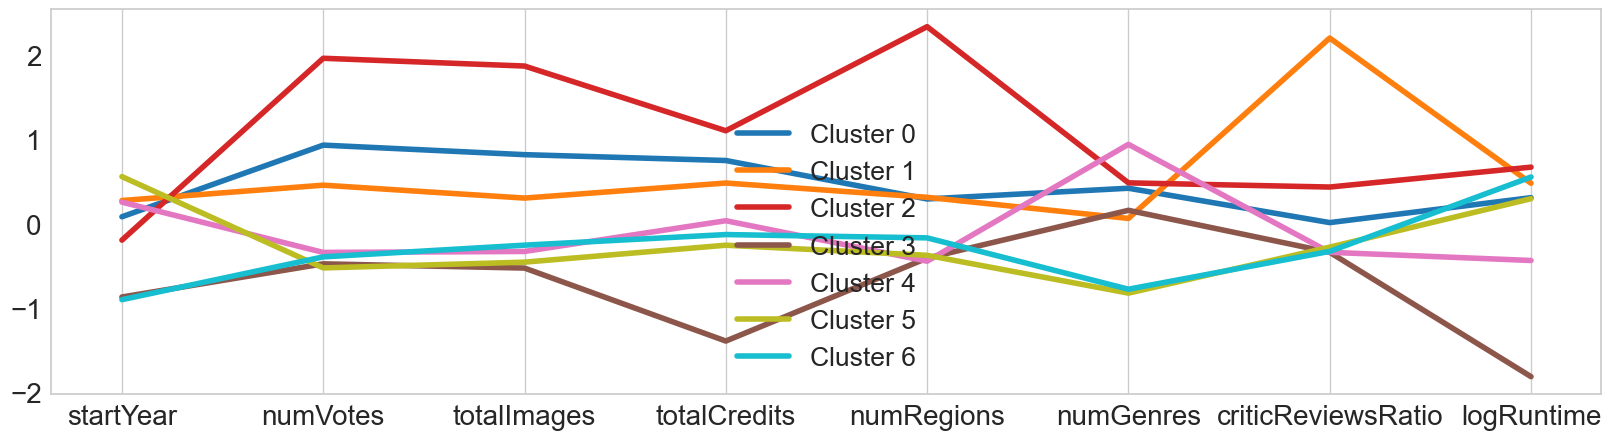
\includegraphics[width=\columnwidth]{../results/images/centroids_bkmeans.png}
    \caption{Centroids' visualization for BK-Means.}
    \label{fig:centroids_bkmeans.png}
\end{figure}

Like for K-Means, we visualized the distribution of the clusters against known categorical features. We find many similarities with the previous algorithm, but also some differences:
\begin{itemize}
    \item \textit{titleType} (cf. Figure \ref{fig:heatmap_titleType_bkmeans.png}): again, the distribution of shorts is what becomes immediately evident. Around half of them are to be found in Cluster 3, which also has a small proportion of tvEpisodes and is the only cluster with almost no movies. Cluster 4, the 2nd biggest cluster, is mostly made of tvEpisodes and a smaller, yet significant, proportion of shorts. The few tvShort recorded are also distributed among these two clusters. It's also worth noting that Cluster 6 contains the biggest number of movies, although being only the 3rd most popular, and that Cluster 2 is the only cluster with almost no tvEpisodes. Cluster 5, the biggest, contains the largest part of the remaning title types (except for videogame, which are mostly in Cluster 4).
    \item Boolean variables: again, the cluster whose centroid had the highest value for \textit{numvotes}, \textit{totalImages}, \textit{totalCredits} and \textit{numRegions}, Cluster 2, also has the highest proportion of True values for \textit{hasVideos} and \textit{awardsAndNominations}, at around 50\%. The biggest cluster has the most True values for \textit{canHaveEpisodes} because it contains most of the series. Cluster 6 has almost no True values for \textit{hasVideos}, probably because it contains older titles.
\end{itemize}
\begin{figure}
    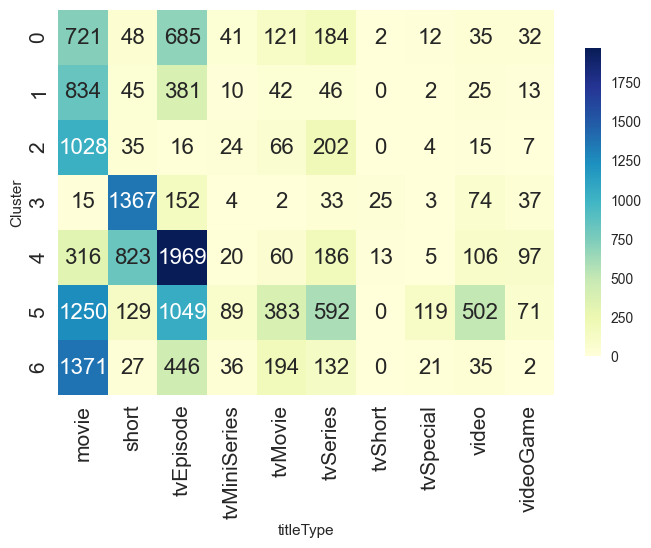
\includegraphics[width=\columnwidth]{../results/images/heatmap_titleType_bkmeans.png}
    \caption{Heatmap Clusters vs titleType (BK-Means).}
    \label{fig:heatmap_titleType_bkmeans.png}
\end{figure}

By visualizing the clusters' composition w.r.t. the numeric variables used by the algorithm, we can see how the line graph for \textit{startYear} (Figure \ref{fig:startYear_bkmeans.png}) shows important differences to the one for K-Means. Cluster 3 (the shorts' cluster) does contain the majority of records released before 1930s, but it actually has titles from all years: we were correct in assuming that it contains both older and newer shorts. Cluster 6 only has records released between the 1910s until 1999, and contains the majority of records released from 1955 until 1987. Cluster 5 (the biggest one) only contains newer titles, released since the 1980s.
W.r.t. \textit{numGenres}, only Cluster 4 has no records with one genre: it contains the largest amount of records with three genres, as well as some with two. Clusters 5 and 6 are also quite pure, with a majority of records with one genre, a minority with two, and a negligible amount with three.
\begin{figure}
    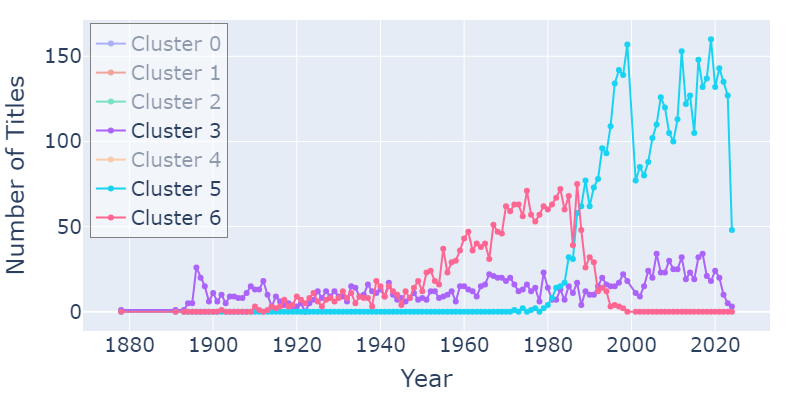
\includegraphics[width=\columnwidth]{../results/images/startYear_bkmeans.png}
    \caption{Number of titles by year for relevant clusters for BK-Means.}
    \label{fig:startYear_bkmeans.png}
\end{figure}

In conclusion, although Bisecting K-Means has yielded worse metrics than K-Means, it has still produced meaningful clusters, comparable to those from K-Means. Both algorithms have created one or two clusters containing shorts, one containing a large portion of tvEpisodes, a cluster containing mainstream/popular content, and one with critically interesting titles. Neither clustering is separated w.r.t the rating (for both, the clusters are normally distributed against \textit{ratingNum}).